
%!TEX root = ./main.tex
%** 50_integration.tex
\chapter{Extending FACT with Server Sockets\label{chapter:integration}}

%%%%%%%%%%%%%%%%%%%%%%%%%%%%%%%%%%%%%%%%%%%%%%%%%%%%%%%%%%%%%%%%%%%%%%%%%%%%%%%%
% Smart Traffic Selection using Server Sockets Sets
%%%%%%%%%%%%%%%%%%%%%%%%%%%%%%%%%%%%%%%%%%%%%%%%%%%%%%%%%%%%%%%%%%%%%%%%%%%%%%%%
\section{Smart Traffic Selection using Server Sockets Sets\label{section:ses_traffic_selection}}
% explain briefly the approach / adjustments to FACT
Originally, FACT applies a port-based heuristic for selecting the examination 
traffic. In detail, FACT selects in a first step all traffic towards an external 
port 80 originated from an internal client high port. Generally, this kind of 
traffic is denoted as the reflector traffic. Then, FACT examines each connection 
from the reflector traffic if it is balanced or unbalanced, thus creating an 
initial set of potential events. 

\begin{figure}
	[!b] \centering
	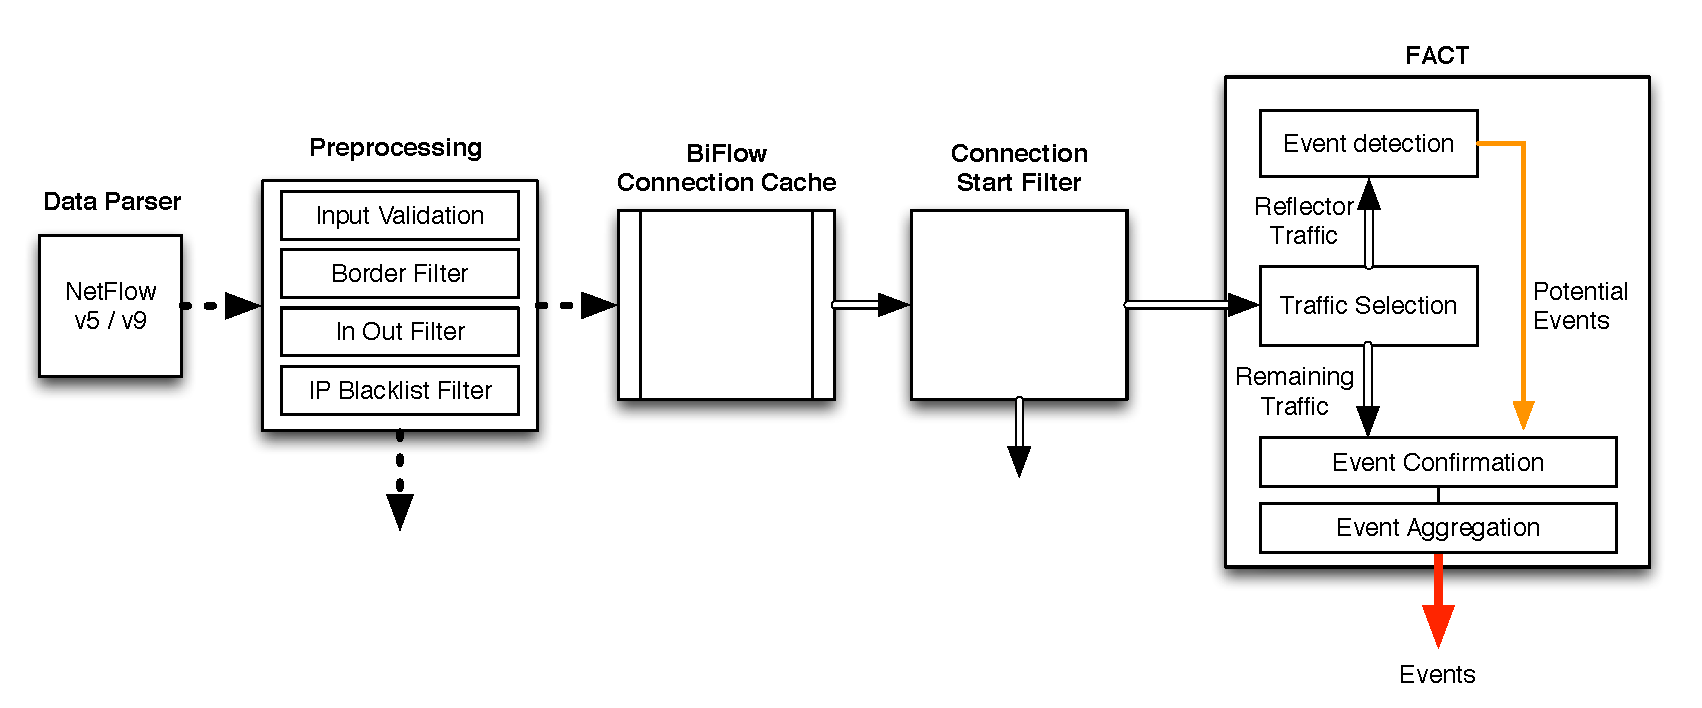
\includegraphics[width=\linewidth]{images/FACT.eps}
	\caption{Processing chain for FACT} 
	\label{fig:fact_chain} 
\end{figure}

In a second step, all unbalanced connections from the reflector traffic are 
double-checked with the remaining traffic if a potential event is indeed a 
event. Only if there are no successful connections at all, i.e. all connections 
are unbalanced, a host, network or prefix is declared as unreachable. Otherwise, 
if there is other traffic towards these hosts, networks, and prefixes with 
balanced connections, the potential event is obviously not confirmed and thus 
removed from the event list. 

Since the server socket approach aims to replace the port-based heuristic, only the generation of the reflector traffic set must be adjusted. The further processing steps remain exactly the same. Figure \ref{fig:fact_chain} illustrates the FACT processing chain and makes clear that only the block of the traffic selection must be adjusted to examine traffic towards server sockets as reflector traffic. This is achieved by loading the server socket registry with a set of server sockets. Then, the adjusted traffic selection is querying the server socket registry if the external socket is a known server socket. If this is the case, the flow is added to the reflector traffic, otherwise to the remaining traffic. 

\section{Optimal Server Sockets Sets\label{section:ses_selection}}
% outline that this is a optimization problem which is approximated by several socket sets however not guaranteed to be optimal
% coverage network space / problem space 